\documentclass[a4paper,spanish]{article}
\usepackage[T1]{fontenc}
\usepackage[spanish]{babel}
\usepackage[utf8]{inputenc}
\usepackage{hyperref}
\usepackage{float}

\title{Visualización de datos genómicos: \textit{circos plot}}
\author{Said Muñoz Montero}

\usepackage{Sweave}
\begin{document}
\input{plot-concordance}

\maketitle

\section{Gráfico de circos}
Uno de los retos para el análisis de datos genómicos radica en la visualización de los datos. Especialmente cuando se tienen datos de diferentes plataformas, es posible generar una gran cantidad de gráficos que por separado no logran ser muy claras.

Una forma sencilla y simple de generar un gráfico de datos genómicos es a través de un gráfico de circos, creado por Martin Kryzywinski. Originalmente los gráficos \textit{circos} fueron desarrollados por \href{https://circos.ca/}{Circos}, este tipo de gráficos no está limitado a información genómica.\cite{krzywinski2009circos}

Los \textit{circos} son especialmente útiles para visualizar datos relacionales con múltiples dimensiones. En el caso de las ciencias ómicas, cada año se aumenta la complejidad en el análisis de los seres vivos, desde genómica, transcriptómica, proteómica, metiloma, etc. El gráfico \textit{circos} permite mostrar un panorama integrativo de muchas de estas plataformas.

\begin{figure}[H]
\centering
\includegraphics{circos_example}
\caption{A) Histograma. B) Ideograma. C)Histograma (invertido). D) \textit{Heatmap}. E) \textit{Links}. F) Resaltados. G) Grids. H) Ticks.}
\end{figure}

Se observa en la figura anterior los diferentes tipos de gráficos que se pueden presentar en un gráfico \textit{circos}. El usuario es libre de elegir lo que más se ajuste al tipo de datos con el que cuente.

Usualmente los circos plot se hacen con Perl, generando una serie de archivos de configuración antes de ver el gráfico. Esta tarea puede ser muy pesada, por lo que se mostrarán dos ejemplos usando \textit{R}.

\subsection{Ejemplo 1}
\label{ejemplo1}

En esta sección aprenderemos las bases de un gráfico de circos utilizando los paquetes de Bioconductor: OmicCircos y RCircos.

Cargamos las librerías que se utilizarán. En caso de que no estén instaladas:

\begin{Schunk}
\begin{Sinput}
> source("http://bioconductor.org/biocLite.R")
> biocLite("RCircos")
> biocLite("OmicCircos")
\end{Sinput}
\end{Schunk}

\begin{Schunk}
\begin{Sinput}
> library("OmicCircos")
> library("RCircos")
\end{Sinput}
\end{Schunk}

Utilizaremos la referencia para el humano llamada "hg19".

\begin{Schunk}
\begin{Sinput}
> data("UCSC.hg19.chr")
> head(UCSC.hg19.chr)
\end{Sinput}
\begin{Soutput}
  chrom chromStart chromEnd   name gieStain
1  chr1          0  2300000 p36.33     gneg
2  chr1    2300000  5300000 p36.32   gpos25
3  chr1    5300000  7100000 p36.31     gneg
4  chr1    7100000  9200000 p36.23   gpos25
5  chr1    9200000 12600000 p36.22     gneg
6  chr1   12600000 16100000 p36.21   gpos50
\end{Soutput}
\end{Schunk}

Se puede observar la estructura de los datos (dataframe), donde las columnas corresponden a: cromosoma, posición inicial, posición final, nombre de la región y tinción, respectivamente. 

Para el primer gráfico necesitamos especificar ciertos parámetros:

\textit{\textbf{chr.exclude}} es una variable, normalmente en forma de vector para indicar los cromosomas que se desean excluir del circos plot. 

\begin{Schunk}
\begin{Sinput}
> chr.exclude <- NULL
\end{Sinput}
\end{Schunk}

\textit{\textbf{cyto.info}} contiene el \textit{dataframe} con la información del genoma que se graficará. Para este ejemplo, la referencia del humano.

\begin{Schunk}
\begin{Sinput}
> cyto.info <- UCSC.hg19.chr
\end{Sinput}
\end{Schunk}

\textit{\textbf{tracks.inside}} indica el número de capas que se graficarán dentro del circos. 

\begin{Schunk}
\begin{Sinput}
> tracks.inside <- 1
\end{Sinput}
\end{Schunk}

\textit{\textbf{tracks.outside}} indica el número de capas que se graficarán afuera del circos.

\begin{Schunk}
\begin{Sinput}
> tracks.outside <- 0
\end{Sinput}
\end{Schunk}

Con la función \textit{RCircos.Set.Core.Components} se configura el entorno gráfico.

\begin{Schunk}
\begin{Sinput}
> RCircos.Set.Core.Components(cyto.info, chr.exclude, tracks.inside, tracks.outside);
\end{Sinput}
\end{Schunk}

Utilizaremos también un dataset de \textit{RCircos}.

\begin{Schunk}
\begin{Sinput}
> data("RCircos.Link.Data")
> head(RCircos.Link.Data)
\end{Sinput}
\begin{Soutput}
  Chromosome chromStart  chromEnd Chromosome.1 chromStart.1 chromEnd.1
1       chr1    8284703   8285399         chr1      8285752    8286389
2       chr1   85980143  85980624         chr7    123161313  123161687
3       chr1  118069850 118070319         chr1    118070329  118070689
4       chr1  167077258 167077658         chr1    169764630  169764965
5       chr1  171671272 171671550         chr1    179790879  179791292
6       chr1  174333479 174333875         chr6    101861516  101861840
\end{Soutput}
\end{Schunk}

Guardamos nuestro gráfico en formato PDF con el siguiente código.

\begin{Schunk}
\begin{Sinput}
> out.file <- "RCircosHelloWorld.pdf";
> pdf(file=out.file, height=8, width=8, compress=TRUE);
\end{Sinput}
\end{Schunk}

Para empezar a dibujar el circos ejecutamos:

\begin{Schunk}
\begin{Sinput}
> RCircos.Set.Plot.Area();
\end{Sinput}
\end{Schunk}

Posteriormente se grafica el ideograma (cariotipo):

\begin{Schunk}
\begin{Sinput}
> RCircos.Chromosome.Ideogram.Plot();
\end{Sinput}
\end{Schunk}

Los \textit{links} se grafican usando:

\begin{Schunk}
\begin{Sinput}
> RCircos.Link.Plot(RCircos.Link.Data, 1, TRUE)
\end{Sinput}
\end{Schunk}

Para poder guardar todo el gráfico en el PDF:

\begin{Schunk}
\begin{Sinput}
> dev.off()
\end{Sinput}
\begin{Soutput}
null device 
          1 
\end{Soutput}
\end{Schunk}

El resultado de todo este primer ejemplo es:

\begin{figure}[H]
\centering
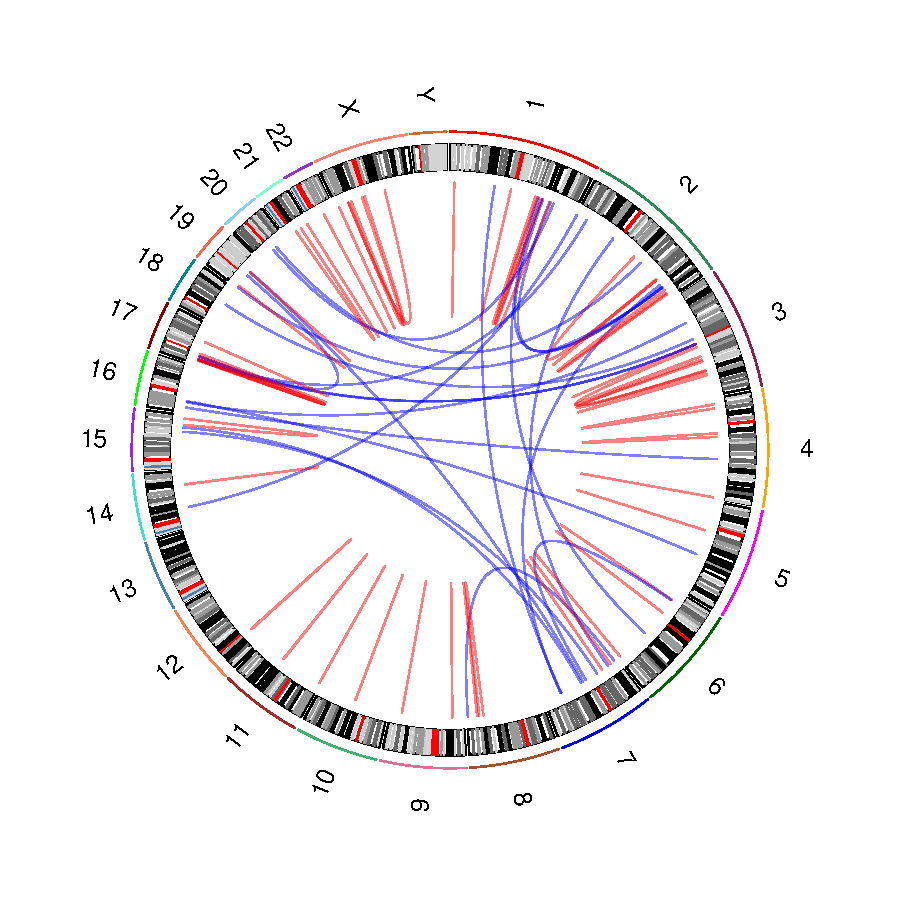
\includegraphics{plot-015}
\caption{Circos plot con Links}
\end{figure}

\subsection{Ejemplo 2}

Para este ejemplo revisaremos el ejemplo de un patógeno intracelular, \textit{Leishmania mexicana}. 

Este organismo cuenta con 34 cromosomas y presenta patrones de expresión, número de copias y genes de fusión muy interesantes.

Dicho esto, utilizamos el genoma de referencia de \textit{Leishmania mexicana}.

En la carpeta de este tutorial se provee el archivo "karyotype.txt".

\begin{Schunk}
\begin{Sinput}
> LmexicanaKaryotype<-read.table("karyotype.txt",header=T)
> head(LmexicanaKaryotype)
\end{Sinput}
\begin{Soutput}
  chrom chromStart chromEnd name stain
1  chr1          0   273339 chr1 black
2  chr2          0   298084 chr2 black
3  chr3          0   376028 chr3 black
4  chr4          0   438911 chr4 black
5  chr5          0   451170 chr5 black
6  chr6          0   479671 chr6 black
\end{Soutput}
\end{Schunk}

Se puede observar una estructura similar al cariotipo humano que se muestra en el ejemplo \ref{ejemplo1}.

Para este ejemplo tenemos que cambiar los parámetros por defecto de las funciones de RCircos.

\begin{Schunk}
\begin{Sinput}
> rcircos.params <- RCircos.Get.Plot.Parameters()
\end{Sinput}
\end{Schunk}

Se modifican las unidades cromosómicas ya que el genoma de \textit{Lmexicana} es más chico al humano. Definimos una unidad cromosómica como 10kbases.
\begin{Schunk}
\begin{Sinput}
> rcircos.params$base.per.unit <- 10000;
\end{Sinput}
\end{Schunk}

De igual forma se ajustan otros parámetros del gráfico.

\begin{Schunk}
\begin{Sinput}
> rcircos.params$chrom.paddings<-10
> RCircos.Set.Core.Components(LmexicanaKaryotype, chr.exclude, tracks.inside, tracks.outside );
> RCircos.Reset.Plot.Parameters(rcircos.params);
> chr.exclude <- NULL;
> tracks.inside <- 3;
> tracks.outside <- 0;
\end{Sinput}
\end{Schunk}

Al igual que en ejemplo \ref{ejemplo1}, generamos un gráfico de cariotipo.


\begin{Schunk}
\begin{Sinput}
> RCircos.Set.Plot.Area();
> RCircos.Chromosome.Ideogram.Plot();
\end{Sinput}
\end{Schunk}

Con \textit{read.table} se carga la matriz de expresión, se observa la estructura de estos datos: cromosoma, posición inicial, posición final y nivel de expresión.

\begin{Schunk}
\begin{Sinput}
> expresion=read.table("expresion.txt",header=T)
> head(expresion)
\end{Sinput}
\begin{Soutput}
  Chromosome Start Final Expression
1       chr1     1   479   0.000000
2       chr1 78487 79506   5.335069
3       chr1 79973 80605   5.973372
4       chr1 81195 81488   6.331023
5       chr1 82545 83321   3.376757
6       chr1 85011 87263   5.122792
\end{Soutput}
\end{Schunk}

Con \textit{RCircos.Line.Plot} se hace una gráfica con los datos de expresión en la primer capa.

\begin{Schunk}
\begin{Sinput}
> RCircos.Line.Plot(expresion,data.col = 4,track.num = 1,side="in")
\end{Sinput}
\end{Schunk}

El archivo "snp.txt", contiene la densidad de mutaciones puntuales promedio en cada cromosoma, esto podría dar una idea del número de copias global de cada cromosoma en este organismo. 

\begin{Schunk}
\begin{Sinput}
> snp=read.table("snp.txt",header=TRUE)
> head(snp)
\end{Sinput}
\begin{Soutput}
  Chromosome   Start   Final   Density
1       chr8 1472001 1473001 0.6696429
2      chr20  464001  465001 0.5357143
3      chr20  465001  466001 0.5267857
4       chr8 1482001 1483001 0.4553571
5      chr20  461001  462001 0.4553571
6       chr8 1466001 1467001 0.4330357
\end{Soutput}
\end{Schunk}

\textit{RCircos.Histogram.Plot} graficará los histogramas de los datos de mutaciones puntuales por cada cromosoma.

\begin{Schunk}
\begin{Sinput}
> RCircos.Histogram.Plot(snp,data.col=4,track.num=2,side="in")
\end{Sinput}
\end{Schunk}

Con secuenciación masiva se lograron determinar genes de fusión en la muestra, se muestran algunos en el archivo "fusiones.txt", y lo graficamos con la misma función usada en el ejemplo \ref{ejemplo1}.

\begin{Schunk}
\begin{Sinput}
> fusiones<-read.table("fusiones.txt",header=TRUE)
> head(fusiones)
\end{Sinput}
\begin{Soutput}
  G1Chromosome G1Start G1Final G2Chromosome G2Start G2Final
1         chr2  238678  238678        chr13   94867   94867
2         chr2  238678  238678        chr13   91780   91780
3         chr2  238678  238678        chr13  119036  119036
4         chr2  238678  238678        chr13  155882  155882
5         chr2  238678  238678        chr13  157632  157632
6         chr2  238678  238678        chr13  398385  398385
\end{Soutput}
\end{Schunk}

\begin{Schunk}
\begin{Sinput}
> RCircos.Link.Plot(fusiones, 3, TRUE);
\end{Sinput}
\end{Schunk}

El resultado es el siguiente:

\begin{figure}[H]
\centering

\includegraphics{plot-plotlm}
\caption{Circos plot para \textit{Leishmania mexicana}}
\end{figure}

\section{Conclusiones}
RCircos es una gran herramienta para generar gráficos exploratorios, sin embargo para generar gráficos más completos se pueden revisar otras implementaciones de Circos plot.

Los gráficos de circos permiten atacar el problema de visualización que aqueja a las ómicas.

\bibliography{bibliography}
\bibliographystyle{plain}
\nocite{*}

\end{document}
